\chapter{Experimental Results}
\label{ch:chapter3}
In order to evaluate the algorithm proposed in Chapter~\ref{ch:chapter2}, in the context of the Leonardo Drone Contest, several experiments where performed. The aim of these experiments were to evaluate:
\begin{itemize}
    \item{the importance of known poles and known and unknown markers in the localization and mapping process}
    \item{the accuracy of markers' pose estimation}
    \item{the importance of the range and Octomap measurements in the height correction}
    \item{the importance of the \ac{NEES} test to evaluate measurements and the filter's consistency}
\end{itemize}
The whole process was tested using \ac{ROS} bags in order to replicate an experiment using different configurations.\\

An important thing to mention is that the ground truth is provided by a Gazebo plug-in, only in a simulated environment. Odometry only, without correction of any kind, is provided as control process and used to compare the results. \\

Figure~\ref{fig:chapter3:odom-only} shows the representation of the odometry used for control purposes, as well as the MAVROS estimate and the ground truth. The figure shows the drift in the MAVROS estimate and in the EKF-SLAM estimate. The yaw estimate follows the ground truth with almost no drift in both MAVROS and EKF-SLAM estimators, while the drone's height does not follow the ground truth at all in the EKF-SLAM process.\\

It is worth to mention that the negative sign in the Z position of the EKF-SLAM process is due to negative velocities in the control signal. This is not something to be concerned about and it is the expected behavior given the linear velocities provided by MAVROS. The positive velocity while the drone takes off is not hold during enough time to position the Z prediction near the ground truth. Furthermore, the linear velocity control signal for the first 25 seconds is negative, which makes the drone "fly below ground". The take off starts at the second 25 and pushes the drone over the ground for some seconds, while the linear velocity published by MAVROS oscillates in between positive and negative values, being the last ones more often. This does not happen with the MAVROS estimator, because it has an own \ac{EKF} filter that produces the Z position estimation. Hence, the comparison in this case is meaningless. The MAVROS \ac{EKF} filter has nothing to do with the motion model in the EKF-SLAM algorithm which does not correct the prediction in any sense.\\

Less is the error in the position estimates in X and Y, where the MAVROS estimation is near the ground truth despite it drifts over time. The EKF-SLAM motion model drifts in a more evident way, both in X and Y: it starts at the same position as the ground truth, but constantly moves away from it. However, and unlike the Z position, both MAVROS and EKF-SLAM motion model follow the ground truth position. Again, comparing the MAVROS estimate with the EKF-SLAM prediction is meaningless as the first one is the result of an \ac{EKF} that uses the measurements provided by the flight controller (IMU, rotors speed, etc.) to predict and update the state, while the second one is composed only by the prediction resulting from the motion model.
\begin{figure}
    \centering
    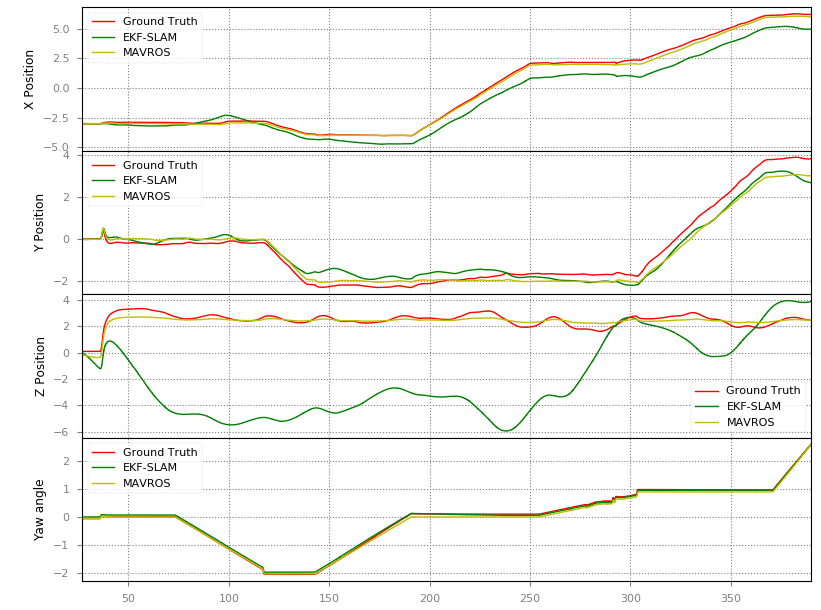
\includegraphics[width=\textwidth]{Images/fig19-odom_only}
    \caption[Odometry only plot]{Odometry only plot. It can be seen three different lines: the red one is the ground truth, the yellow one is the MAVROS estimate and the green one is the EKF-SLAM motion model presented in this work.}
    \label{fig:chapter3:odom-only}
\end{figure}

\section{The Environment}
\label{sec:chapter3:environment}
The simulated environment can be seen in Figure~\ref{fig:chapter3:env:gazebo}, where all the obstacles, poles and markers are disposed. Moreover, the walls define the limits of the environment, making it impossible to go off the limits. The markers were disposed arbitrarily around the world, while the poles are in the same place as they should be in the competition: one in each corner, and two along the middle axis of the space.
\begin{figure}
\centering
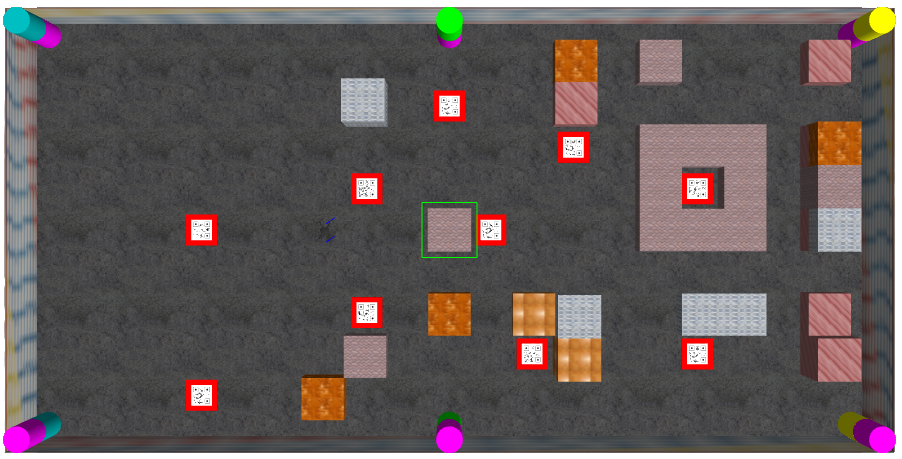
\includegraphics[width=\textwidth]{Images/fig18-gazebo-environment}
\caption{Gazebo simulated environment.}
\label{fig:chapter3:env:gazebo}
\end{figure}
The drone is placed at coordinates $(-3;0)$, and can be depicted in the figure as the green circle in the middle left. As mentioned before, the poles have a different combination of colors, where two poles do not have the same combination. The markers, are QR codes framed in red, while obstacles are brown and gray boxes around the environment. The walls are made of a net-like material distinguishable from the obstacles, while the floor is a pavement-like material.

\section{Simulated Experiments}
\label{sec:chapter3:simulation}
The following experiments were done using a simulated environment. The system was run and a \ac{ROS} bag was recorded in order to analyze different aspects of the environment using the same simulation, and therefore, being able to compare between different configurations. Noise tuning was done empirically using the \ac{ROS} bag in order to obtain the best possible results, while taking into consideration the fact that noise values have a physical meaning.\\

Four sets of experiments with different objectives were conducted:
\begin{enumerate}[a)]
    \item{\textbf{Experiments A}: These experiments aim to show the importance of poles in the localization process.}
    \item{\textbf{Experiments B}: These experiments aim to show the importance of markers in the localization and mapping process.}
    \item{\textbf{Experiments C}: These experiments aim to show the importance of the range sensor in the estimation of the drone's height.}
    \item{\textbf{Experiments D}: These experiments aim to understand the importance of the \ac{NEES} test in the acceptance of the observations.}
\end{enumerate}
All these experiments were carried out using the same bag, unless the contrary is mentioned.

\subsection{Experiments A: The importance of poles}
\label{subsec:chapter3:simulation:a}
The experiments presented in this section were done with the objective of understanding the importance of poles in the localization of the drone in the environment. Two experiments were performed: the first experiment was carried out with perfect observations of poles, while the second experiment was carried out using the real measurements taken from the \ac{ROS} bag.

\subsubsection{Procedures}
\label{subsubsec:chapter3:simulation:a:procedures}
As mentioned, the first experiment was performed with perfect observations of poles, with the objective of showing the perfect localization compared with the MAVROS localization and the ground truth. On the other hand, the second experiment was performed with the real observations taken from the \ac{ROS} bag, in order to understand if the proposed implementation works as well as with the perfect observations of the previous experiment.\\

In these experiments the same \ac{ROS} bag is used, and the measurements are taken during approximately 360 seconds. During the path, the drone visits few markers and pass over some obstacles, both of which are not taken into account in the localization process.

\subsubsection{Results}
\label{subsubsec:chapter3:simulation:a:results}
The results in these experiments are shown in Figure~\ref{fig:chapter3:simulation:experimentsA:a} for perfect pole observations and in Figure~\ref{fig:chapter3:simulation:experimentsA:b} for real poles observations. With respect to the first experiment, it can be said that the correction is almost perfect as the path followed by the drone follows the ground truth all the time. However, and as it is expected, in the second experiment the EKF-SLAM estimation follows the ground truth but with more noise than in the previous one. There are some moments in which the estimation is more noisy than usual: this has to do with occlusions and far-from-true measurements.
\begin{figure}
    \centering
    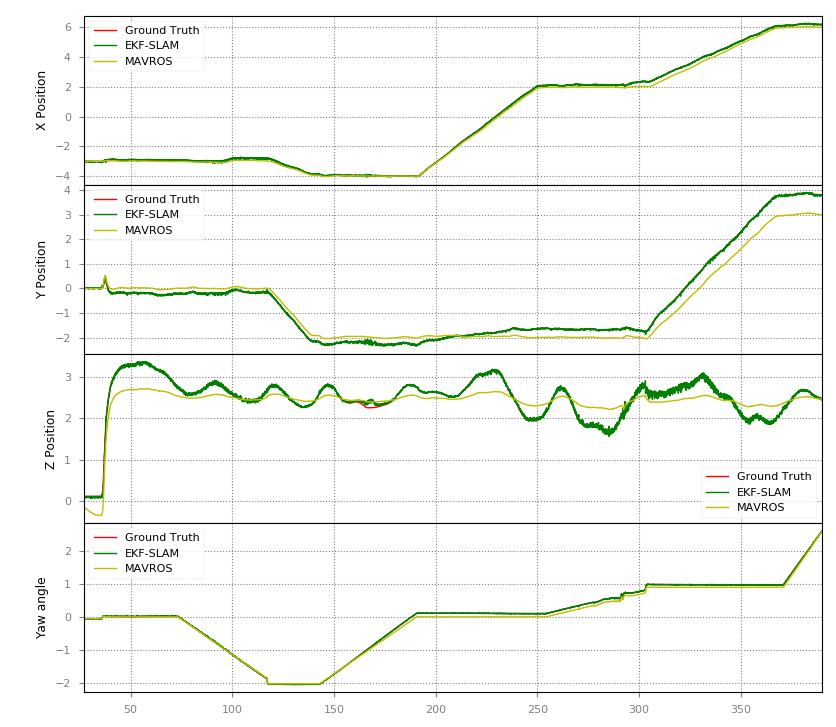
\includegraphics[width=\textwidth]{Images/fig20-exp-a1}
    \caption{Localization using perfect pole observations.}
    \label{fig:chapter3:simulation:experimentsA:a}
    \centering
    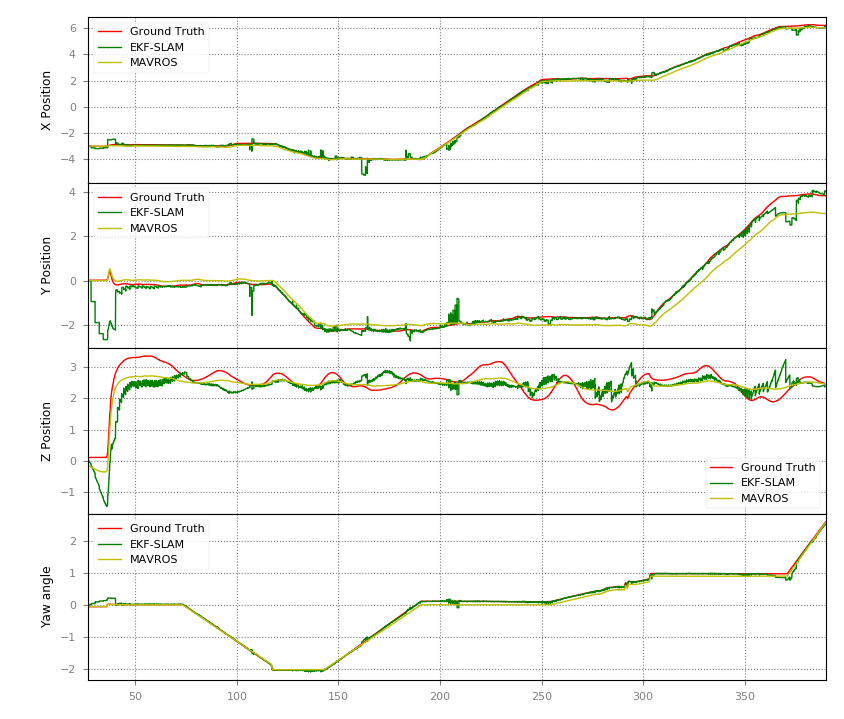
\includegraphics[width=\textwidth]{Images/fig20-exp-a2}
    \caption{Localization using real pole observations.}
    \label{fig:chapter3:simulation:experimentsA:b}
\end{figure}

\subsection{Experiments B: The importance of markers}
\label{subsec:chapter3:simulation:b}
Differently from poles, markers are sporadically seen, and therefore, it can be assumed that its contribution to the localization will be sparse. On the other hand, one can imagine that using poles and markers for localization-only purposes will improve the estimation seen in Figure~\ref{fig:chapter3:simulation:experimentsA:b}.\\

A set of different experiments were carried out in this section, and all of them aim to understand the importance of markers during the localization. On the other hand, a subset of these experiments try to measure the mapping process and the mapping process jointly with the localization.

\subsubsection{Procedures}
\label{subsubsec:chapter3:simulation:b:procedures}
The experiments presented in this section were carried out using the same \ac{ROS} bag. The difference between them lies on the usage or not of real markers' observations, and lies on the usage or not of a previously built map of markers.\\

The experiments conducted are the followings:
\begin{enumerate}
    \item{The first experiment is similar to the ones presented in Section~\ref{subsec:chapter3:simulation:a}. The drone follows the path and estimates its pose based on known markers only. This means that the drone performs only the localization, and no marker is added to the map.}
    \item{The second experiment is similar to the previous one, but it uses markers and poles to localize. However, the main difference with the previous experiments lies on the absence or not of a perfect map. This means that when the map is not available, the algorithm will create it, while if the map is available, the algorithm will use it to update the drone's pose.}
    \item{Finally, the third experiment measures the distance between the true position of markers and the one estimated by the algorithm in a context of real observations, both for markers and poles.}
\end{enumerate}

\subsubsection{Results}
\label{subsubsec:chapter3:simulation:b:results}
The first set of experiments related to the markers, aim to identify the marker's importance in the localization problem. Two plots are presented to this purpose, and are shown in Figure~\ref{fig:chapter3:simulation:b:fake-markers-real-map} and Figure~\ref{fig:chapter3:simulation:b:real-markers-real-map}. Figure~\ref{fig:chapter3:simulation:b:fake-markers-real-map} shows the path followed by the drone while using only the perfect observations of markers and a perfect map, while Figure~\ref{fig:chapter3:simulation:b:real-markers-real-map} shows the path followed while using real observations of markers with a perfect map. Having a perfect map means that the markers' poses are perfectly known, hence the true position and orientation is given to the algorithm. \\
\begin{figure}
    \centering
    \begin{subfigure}{\textwidth}
        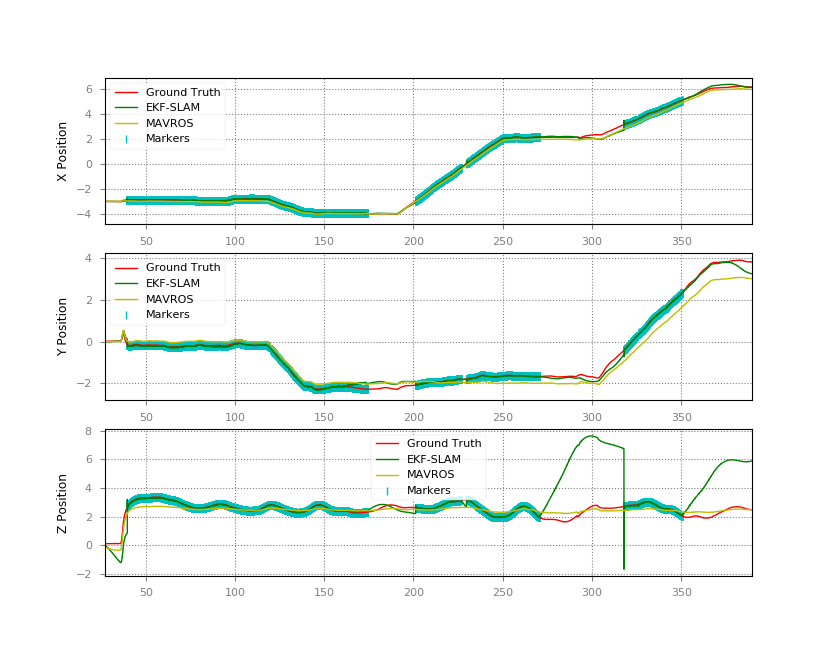
\includegraphics[width=1\linewidth]{Images/fig21-fake-markers-wmap.png}
        \caption{Localization with perfect marker observations}
        \label{fig:chapter3:simulation:b:fake-markers-real-map}
    \end{subfigure}
    \begin{subfigure}{\textwidth}
        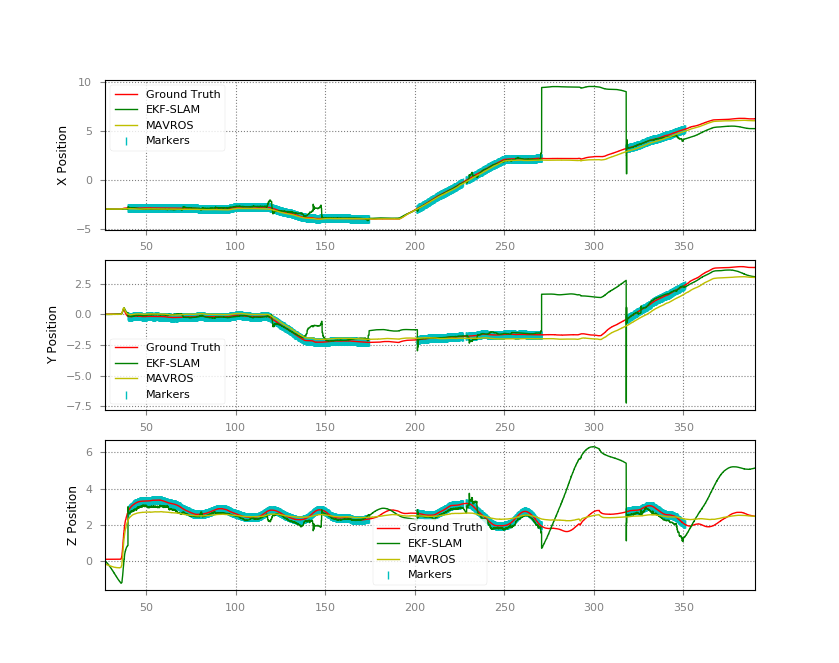
\includegraphics[width=1\linewidth]{Images/fig21-real-marker-wmap.png}
        \caption{Localization with real marker observations}
        \label{fig:chapter3:simulation:b:real-markers-real-map}
    \end{subfigure}
    \caption[Localization with perfect and real marker observations]{Localization with perfect \textbf{(a)} and real \textbf{(b)} marker observations. Between seconds 180 and 220, seconds 260 and 320, and from second 350 to the end, no marker is seen producing huge errors in the estimate.}
\end{figure}

It can be seen in both figures that, even if the path taken by the drone does not follow perfectly the ground truth, it accommodates when it sees a marker. This behavior can be appreciated between seconds 180 and 220, and can be seen in Figure~\ref{fig:chapter3:simulation:b:real-markers-correction-detail}.\\
\begin{figure}
    \centering
    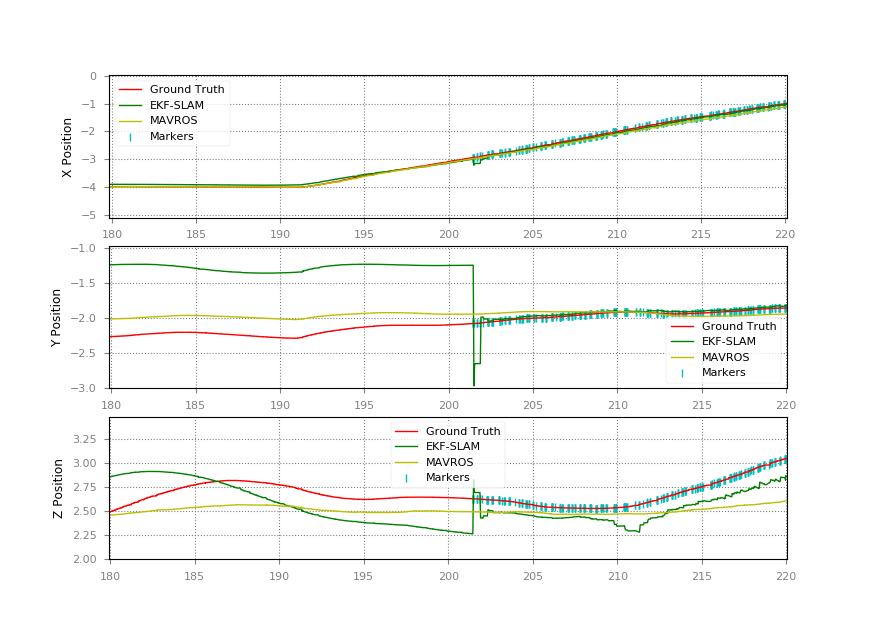
\includegraphics[width=0.9\textwidth]{Images/fig21-real-marker-wmap-correction-detail.png}
    \caption[Detail of correction process with markers.]{Detail of correction process in the case of markers-only localization. As soon as the drone visualizes a marker, it corrects its pose according to the observation.}
    \label{fig:chapter3:simulation:b:real-markers-correction-detail}
\end{figure}

The second set of experiments was designed to understand the importance of markers and poles in the localization problem. In this case, the drone follows the path and corrects its position using known poles and unknown markers. As can be seen in Figure~\ref{fig:chapter3:simulation:b:real-poles-fake-markers-real-map} and Figure~\ref{fig:chapter3:simulation:b:real-poles-markers-real-map}, the drone follows the path almost perfectly, and gets lost in the periods where it does not see any marker. However, as the algorithm uses both poles and markers to update the drone's pose, it does not diverge when no marker is seen, making the estimation more robust in these situations. The difference between Figure~\ref{fig:chapter3:simulation:b:real-poles-fake-markers-real-map} and Figure~\ref{fig:chapter3:simulation:b:real-poles-markers-real-map} is that, in the first one perfect markers are seen, while in the second one real markers are seen. This is particularly evident between seconds 130 and 150, where accepted observations that are far from the true marker position, make the filter to diverge from the ground truth. Insight into this problem will be discussed later on in this chapter.\\
\begin{figure}
    \centering
    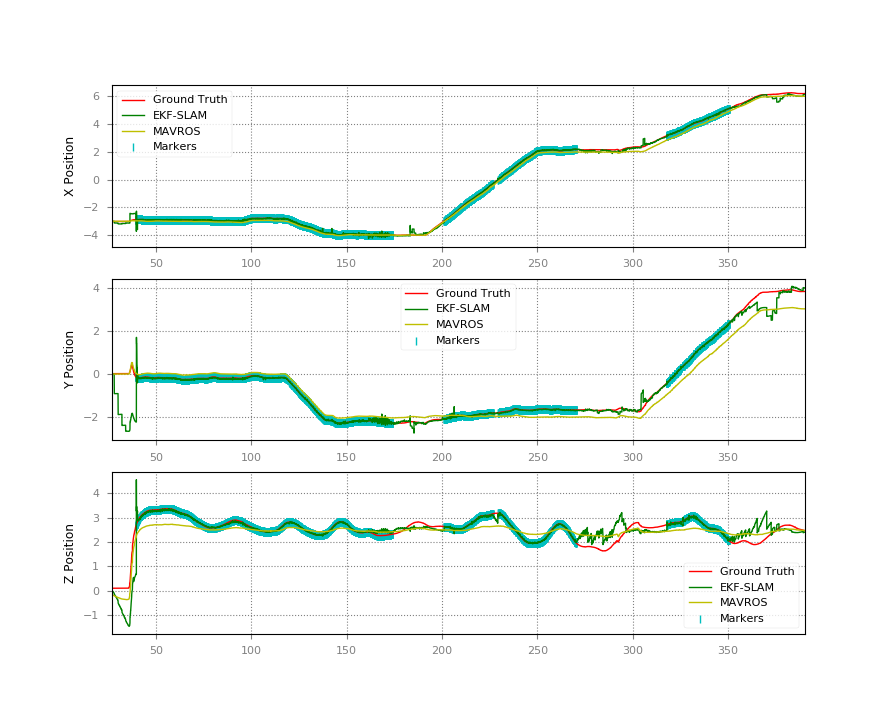
\includegraphics[width=\textwidth]{Images/fig22-true-poles-fake-markers-wmap.png}
    \caption{Localization using real pole observations and perfect marker observations.}
    \label{fig:chapter3:simulation:b:real-poles-fake-markers-real-map}
    \centering
    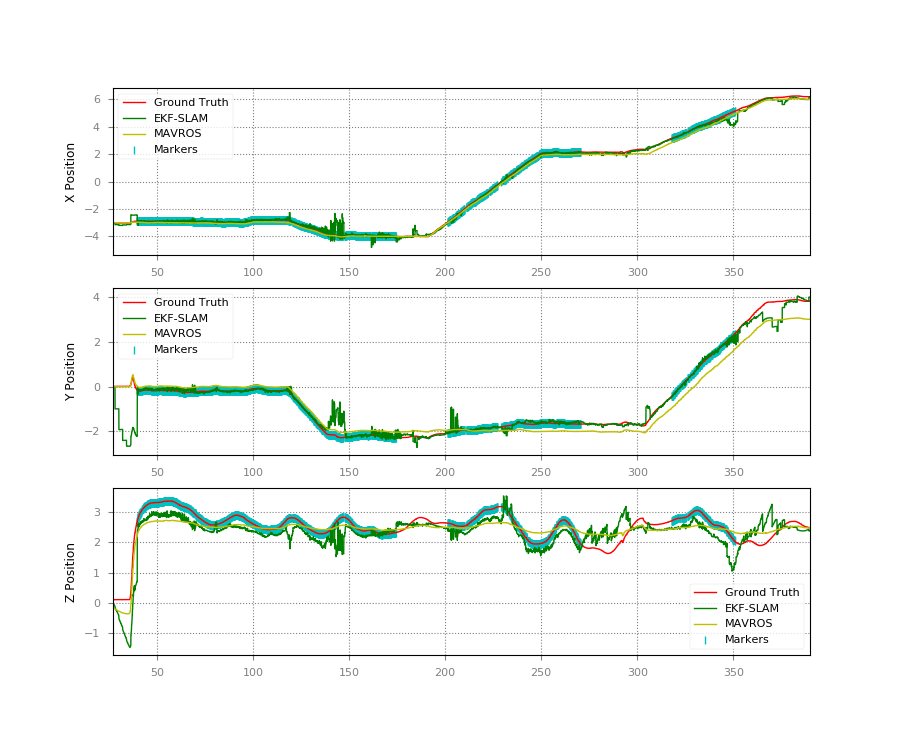
\includegraphics[width=\textwidth]{Images/fig22-true-poles-markers-wmap.png}
    \caption{Localization using real pole and real marker observations.}
    \label{fig:chapter3:simulation:b:real-poles-markers-real-map}
\end{figure}

Something worth understanding is how different is the localization process when the map is available, and when it is not. So far, the experiments shown were developed using a map with the true pose of markers. However, this is not always possible, and since \ac{SLAM} is a two step problem (mapping and localization), a map needs to be built first. In the Figure~\ref{fig:chapter3:simulation:b:real-poles-markers-no-map} it can be seen the state estimation when no map is available, and real observations of both poles and markers are used. When comparing Figure~\ref{fig:chapter3:simulation:b:real-poles-markers-no-map} with Figure~\ref{fig:chapter3:simulation:b:real-poles-markers-real-map} no big differences can be appreciated.\\
\begin{figure}
    \centering
    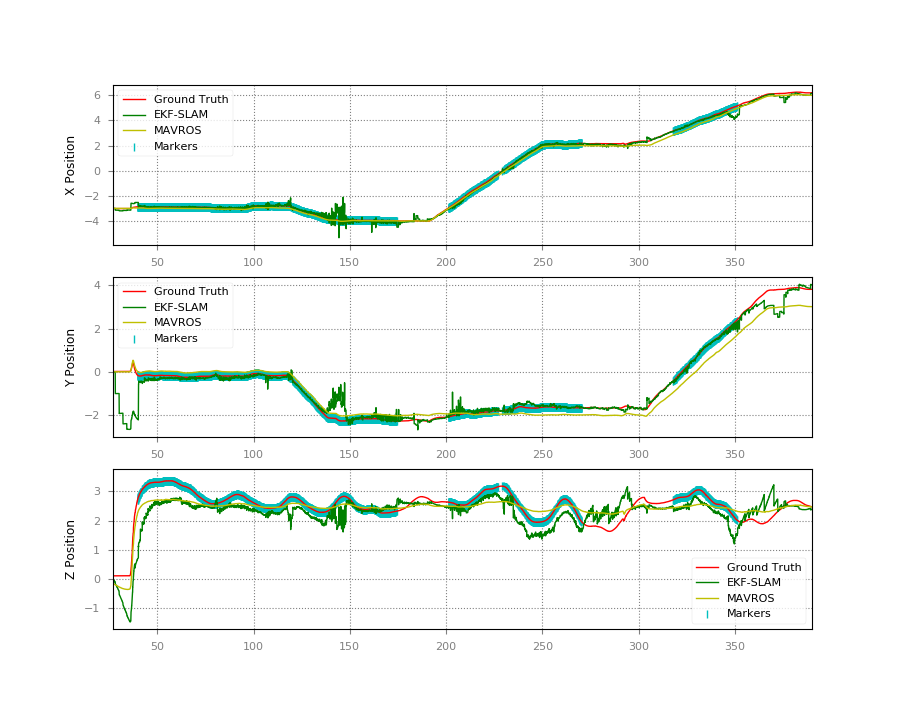
\includegraphics[width=\textwidth]{Images/fig22-true-poles-markers-nomap.png}
    \caption[Simultaneous localization and mapping using real pole and marker observations.]{Simultaneous localization and mapping using real pole and marker observations. The EKF-SLAM algorithm estimates the drone's pose while building a map from unknown markers' observations.}
    \label{fig:chapter3:simulation:b:real-poles-markers-no-map}
\end{figure}

Finally, the last set of experiments measure the distance between the true markers' pose and the one estimated by the algorithm. The Euclidean distance (in meters) is calculated for the position of the markers, and the orientation is shown as the relative rotation, needed to go from the estimated one to the true one, expressed as $\phi$, $\theta$ and $\psi$ (in radians). The Euclidean distance is defined as\\
\begin{equation*}
    D = \sqrt{(x - \hat{x})^2 + (y - \hat{y})^2 + (z - \hat{z})^2}~~.
\end{equation*}
The results for those markers seen during the drone's path are presented in Table~\ref{tab:chapter3:simulated:experiments:b:distance}. The estimated pose and the ground truth can be seen in the Table~\ref{tab:chapter3:simulated:experiments:b:poses}. It is worth mentioning that more than the 60\% of the markers' observations were accepted by the \ac{NEES} test, and thus were considered for updating the state:
\begin{itemize}
    \item{\textbf{Marker 0}: 69.36\%}
    \item{\textbf{Marker 1}: 65.68\%}
    \item{\textbf{Marker 4}: 70.21\%}
    \item{\textbf{Marker 5}: 67.94\%}
\end{itemize}

\begin{table}
    \centering
    \begin{tabular}{ccccc}
        \toprule
        \textsc{Marker ID} & \textsc{Euclidean distance} & \textsc{$\phi$} & \textsc{$\theta$} & \textsc{$\psi$} \\
        \midrule
        0 & 0.076 & 0.089 & 0.142 & 0.034\\
        1 & 0.186 & 0.407 & 0.145 & 0.052\\
        4 & 0.119 & 0.153 & 0.132 & 0.055\\
        5 & 0.155 & 0.024 & 0.057 & 0.013\\
        \bottomrule
    \end{tabular}
    \caption[Distance to true markers' pose]{Distance between true markers' pose and the pose estimated by the EKF-SLAM algorithm. The Euclidean distance between markers is expressed in meters, while the distance between orientations is expressed in radians.}
    \label{tab:chapter3:simulated:experiments:b:distance}
\end{table}

\begin{table}
    \centering
    \begin{tabular}{ccccccc}
        \toprule
        \textsc{Marker ID} & X & Y & Z & $\phi$ & $\theta$ & $\psi$ \\
        \midrule
        \multirow{2}{*}{0} & \textcolor{OliveGreen}{-2.0}& \textcolor{OliveGreen}{1.0}& \textcolor{OliveGreen}{0.1}& \textcolor{OliveGreen}{0.0}& \textcolor{OliveGreen}{0.0}& \textcolor{OliveGreen}{-3.142}\\
        & \textcolor{blue}{-2.005}& \textcolor{blue}{0.948}& \textcolor{blue}{0.044}& \textcolor{blue}{-0.088}& \textcolor{blue}{-0.142}& \textcolor{blue}{-3.108}\\
        \midrule
        \multirow{2}{*}{1} & \textcolor{OliveGreen}{3.0}& \textcolor{OliveGreen}{2.0}& \textcolor{OliveGreen}{0.1}& \textcolor{OliveGreen}{0.0}& \textcolor{OliveGreen}{0.0}& \textcolor{OliveGreen}{3.142}\\
        & \textcolor{blue}{3.138}& \textcolor{blue}{1.980}& \textcolor{blue}{0.223}& \textcolor{blue}{-0.407}& \textcolor{blue}{0.145}& \textcolor{blue}{3.089}\\
        \midrule
        \multirow{2}{*}{4} & \textcolor{OliveGreen}{-2.0}& \textcolor{OliveGreen}{-2.0}& \textcolor{OliveGreen}{0.1}& \textcolor{OliveGreen}{0.0}& \textcolor{OliveGreen}{0.0}& \textcolor{OliveGreen}{-3.142}\\
        & \textcolor{blue}{-2.070}& \textcolor{blue}{-1.912}& \textcolor{blue}{0.062}& \textcolor{blue}{0.153}& \textcolor{blue}{0.132}& \textcolor{blue}{-3.087}\\
        \midrule
        \multirow{2}{*}{5} & \textcolor{OliveGreen}{1.0}& \textcolor{OliveGreen}{0.0}& \textcolor{OliveGreen}{0.1}& \textcolor{OliveGreen}{0.0}& \textcolor{OliveGreen}{0.0}& \textcolor{OliveGreen}{3.142}\\
        & \textcolor{blue}{1.040}& \textcolor{blue}{-0.053}& \textcolor{blue}{-0.040}& \textcolor{blue}{-0.024}& \textcolor{blue}{0.057}& \textcolor{blue}{3.128}\\
        \bottomrule
    \end{tabular}
    \caption[Marker's estimated pose]{Marker's estimated pose (blue) and marker's real pose (green) comparison.}
    \label{tab:chapter3:simulated:experiments:b:poses}
\end{table}

\subsection{Experiments C: The height estimation}
\label{subsec:chapter3:simulation:c}
The height estimation of the drone is composed by two types of observations: the Octomap generated based on the data provided by the front stereo camera, and the range sensor measurements provided by the Pix4Flow device. The proposed implementation takes care of this, with the solely condition that the Octomap is complete at the current coordinates of the drone, and in that case, the measurement is accepted and the correction step is triggered. \\

The experiment conducted in this section shows the importance of the height correction using both the Octomap and the range sensor measurements, but also, the importance of a well defined Octomap in order to avoid false positives.

\subsubsection{Procedures}
\label{subsubsec:chapter3:simulation:c:procedures}
As with the previous experiments, this one was performed using a \ac{ROS} bag with the range sensor and Octomap information. The drone follows the same path as before, but this time using both measurements to correct its height. % In this case, the drone uses

\subsubsection{Results}
\label{subsubsec:chapter3:simulation:c:results}
The path followed by the robot can be seen in Figure~\ref{fig:chapter3:simulation:c:path-w-range}. The plots are similar to those in Figure~\ref{fig:chapter3:simulation:b:real-poles-markers-real-map}, however the height estimation is different from around second 250. After this second, the Octomap information is available and the correction step in the EKF-SLAM algorithm is triggered.\\
\begin{figure}
    \centering
    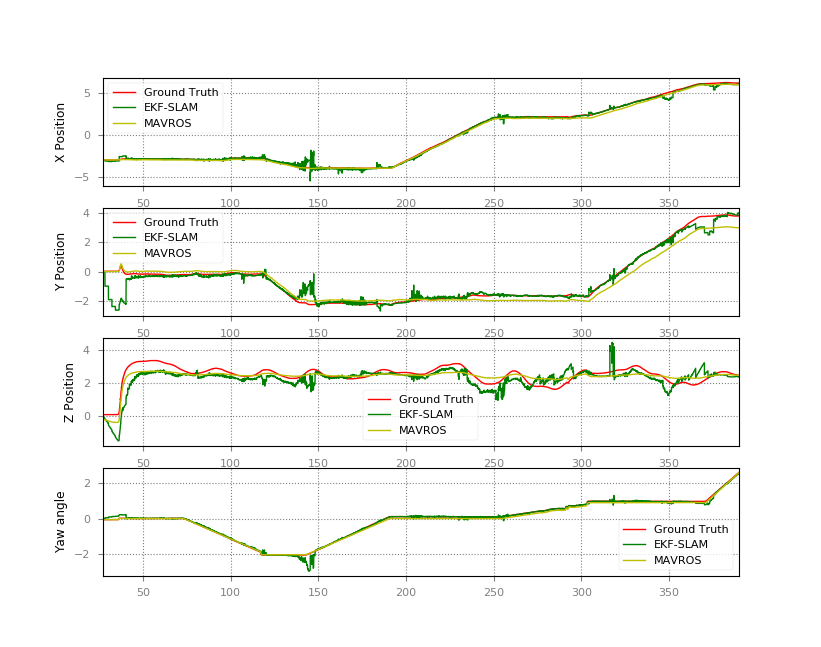
\includegraphics[width=0.9\textwidth]{Images/fig23-path-w-laser.png}
    \caption{Path followed by the drone when correction of height is used.}
    \label{fig:chapter3:simulation:c:path-w-range}
\end{figure}

Figure~\ref{fig:chapter3:simulation:c:range-sensor} shows the same plot as before, with the aggregation of the range sensor information. It can be seen that the drone flew over few obstacles, and the range sensor outputs heights below the ground truth. Accepted and discarded measurements can be appreciated in detail in Figure~\ref{fig:chapter3:simulation:c:range-sensor-detail}, and some interesting conclusions can be deducted. \\

First of all, having an incomplete or noisy Octomap makes the altitude estimation to reach wrong values, as can be seen between seconds 315 to 320. During this 5 seconds, the Octomap returns values near 2.5 meters for the voxels below the drone while the range sensor returns similar values, this makes the algorithm to estimate the Z position to up to 4 meters.\\
\begin{figure}
    \centering
    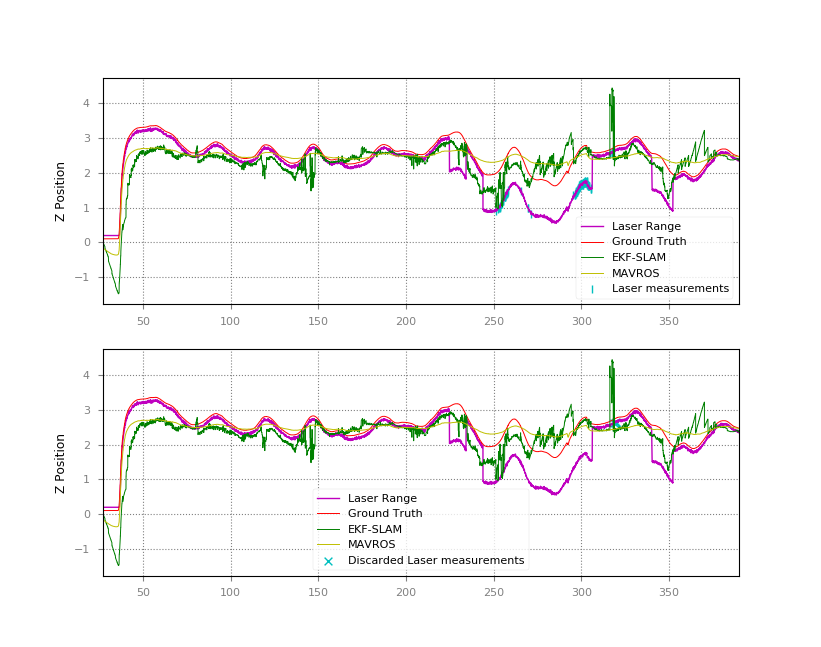
\includegraphics[width=0.9\textwidth]{Images/fig23-laser.png}
    \caption[Height estimation aggregated with range sensor information]{Height estimation aggregated with range sensor information. This plot shows the accepted and discarded observations in the height estimation.}
    \label{fig:chapter3:simulation:c:range-sensor}
    \centering
    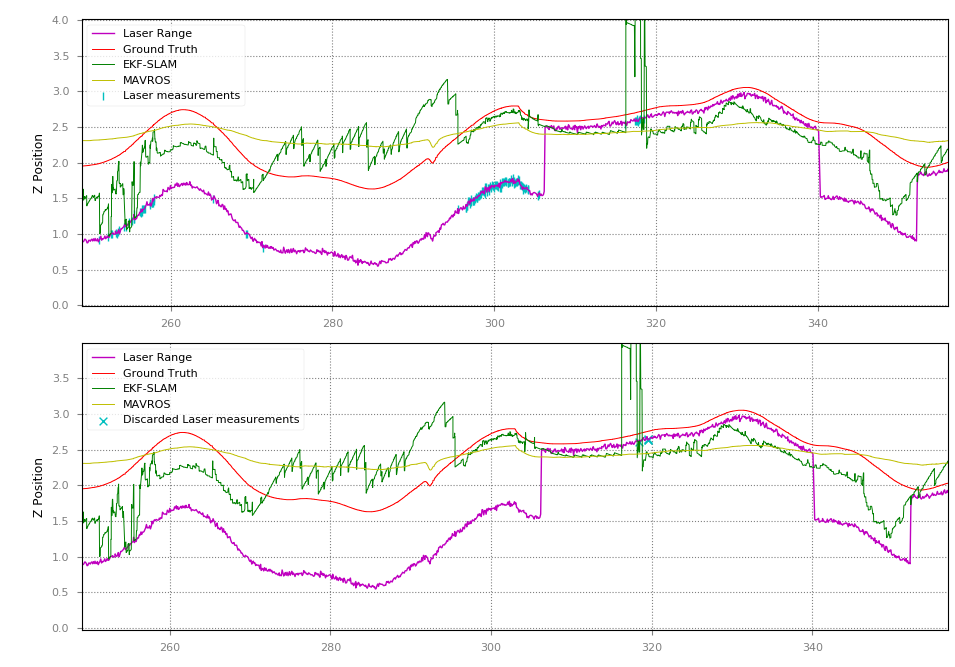
\includegraphics[width=0.9\textwidth]{Images/fig23-laser-detail.png}
    \caption[Detail of height estimation aggregated with range sensor information]{Detail of height estimation aggregated with range sensor information. This plot shows the detail of accepted and discarded observations when the Octomap is available and the Z position correction is triggered.}
    \label{fig:chapter3:simulation:c:range-sensor-detail}
\end{figure}

On the other hand, when the Octomap returns values that are near the ground truth and the drone is over an object, the estimate approaches the ground truth. This can be seen between seconds 295 to 305, where the accepted measurements make the EKF-SLAM algorithm to follow the ground truth.

\subsection{Experiments D: The importance of NEES test}
\label{subsec:chapter3:simulation:d}
Explained in Section~\ref{sec:chapter2:nees}, the \ac{NEES} test helps to the consistency of the filter. In the proposed implementation, the \ac{NEES} test helps to discard measurements too far from the estimated ones, and to accept those that are close to the expected.\\

The experiments in this section are divided in two, and try to shed some light over the following:
\begin{enumerate}
    \item{The importance of using (or not) the \ac{NEES} test}
    \item{The importance of the $\chi^2$ value}
\end{enumerate}

\subsubsection{Procedures}
\label{subsubsec:chapter3:simulation:d:procedures}
Two experiments were conducted using the same \ac{ROS} bag as before, using the real observations for poles and markers and using the measurements of the range sensor for the height estimation. Moreover, the path was followed using localization only with a perfect map. The difference between these two experiments lies on the usage or not of the \ac{NEES} test to discard observations.

\subsubsection{Results}
\label{subsubsec:chapter3:simulation:d:results}
With respect to the importance of the usage of \ac{NEES} test the Figure~\ref{fig:chapter3:simulation:d:no-nees-test} shows the estimation of position in X, Y, Z and $\psi$ when no \ac{NEES} test is applied. This means that all the observations are used to update the state vector. It is evident from Figure~\ref{fig:chapter3:simulation:d:no-nees-test} that without the \ac{NEES} test to filter out the measurements far from the expected, makes the EKF-SLAM algorithm inconsistent.\\
\begin{figure}
    \centering
    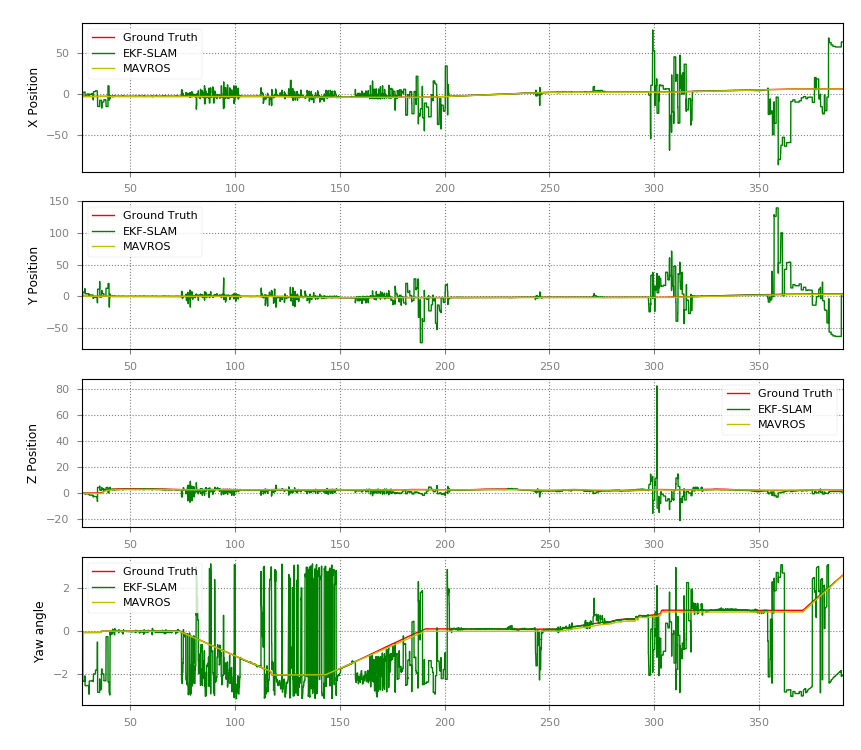
\includegraphics[width=0.9\textwidth]{Images/fig24-no-nees-test.png}
    \caption[EKF-SLAM behavior when NEES test is not used.]{EKF-SLAM behavior when \ac{NEES} test is not used.}
    \label{fig:chapter3:simulation:d:no-nees-test}
    \centering
    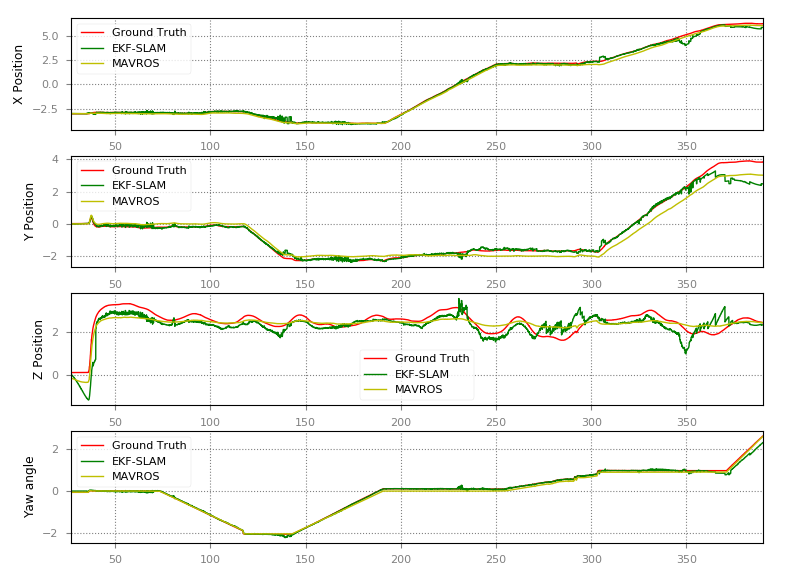
\includegraphics[width=0.9\textwidth]{Images/fig24-nees-10-path.png}
    \caption[EKF-SLAM behavior when $\chi_{\alpha=0.9}^2$]{EKF-SLAM behavior when $\chi_{\alpha=0.9}^2$ corresponding of a 10\% of valid observations.}
    \label{fig:chapter3:simulation:d:nees-10}
\end{figure}

On the other hand, the second experiment aims to find good values for the $\chi^2$ threshold, and therefore, its importance. The results presented so far have used $\chi^2$ values that corresponds to $\alpha=0.05$, therefore a 95\% of confidence that the measurements are valid. However, different results can be achieve if the threshold value changes, as shown in Figure~\ref{fig:chapter3:simulation:d:nees-10} where a value of $\alpha=0.9$, which corresponds of a confidence of 10\% that the measurements are valid, is shown.\\

This change produces an increment in the discarded observations, as it can be seen in Figure~\ref{fig:chapter3:simulation:d:nees-95-discarded-markers} and Figure~\ref{fig:chapter3:simulation:d:nees-10-discarded-markers} for markers. As shown in Figure~\ref{fig:chapter3:simulation:d:nees-10-discarded-markers} the issue commented in Section~\ref{subsubsec:chapter3:simulation:b:results} around seconds 130 and 150 has vanished because those accepted measurements are discarded with the new configuration.\\
\begin{figure}
    \centering
    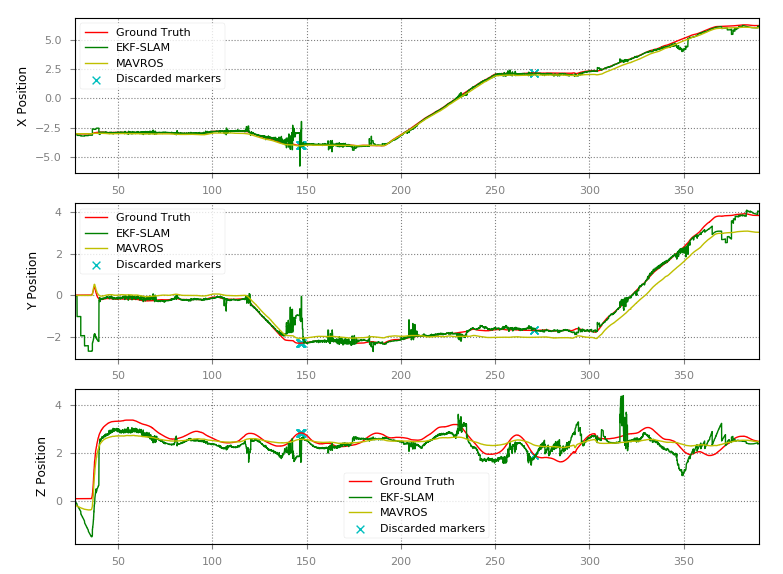
\includegraphics[width=0.9\textwidth]{Images/fig24-nees-95-path-discarded-markers.png}
    \caption[Discarded marker observations when $\chi_{\alpha=0.05}^2$]{Discarded marker observations when $\chi_{\alpha=0.05}^2$ corresponding of a 95\% of valid observations.}
    \label{fig:chapter3:simulation:d:nees-95-discarded-markers}
    \centering
    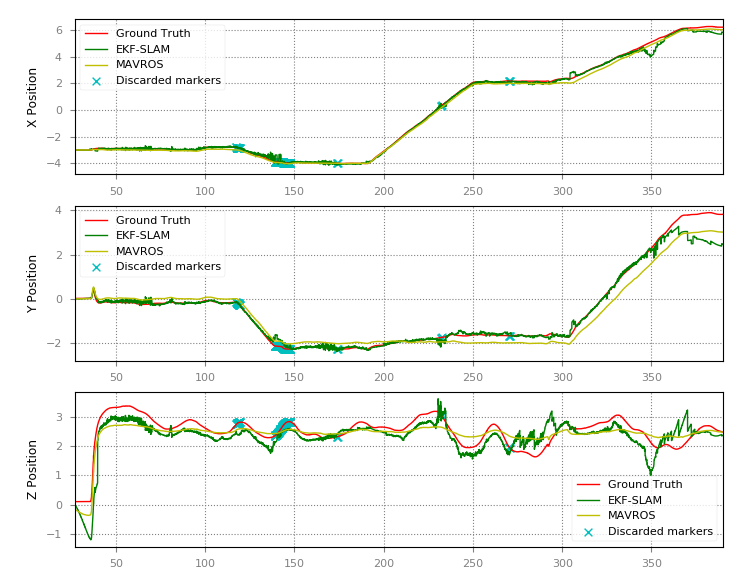
\includegraphics[width=0.9\textwidth]{Images/fig24-nees-10-path-discarded-markers.png}
    \caption[Discarded marker observations when $\chi_{\alpha=0.9}^2$]{Discarded marker observations when $\chi_{\alpha=0.9}^2$ corresponding of a 10\% of valid observations.}
    \label{fig:chapter3:simulation:d:nees-10-discarded-markers}
\end{figure}

\begin{figure}
    \centering
    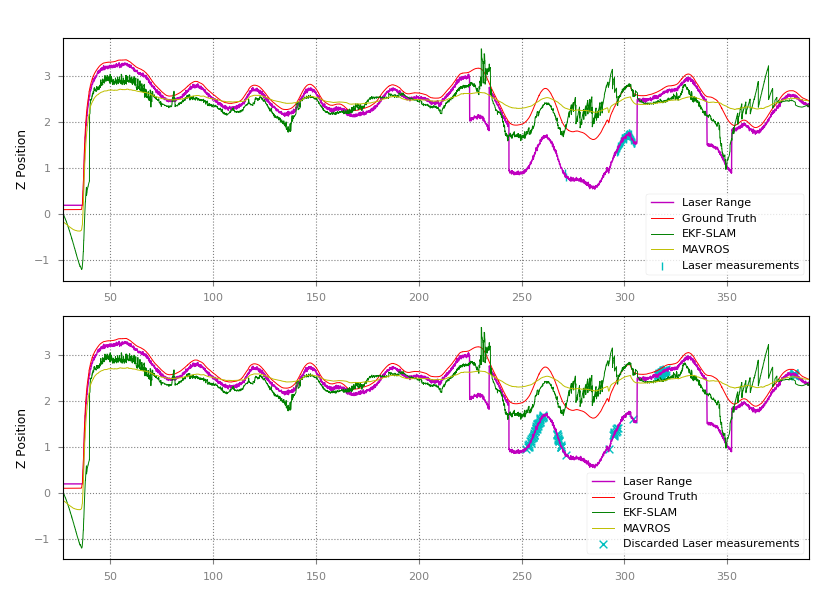
\includegraphics[width=0.9\textwidth]{Images/fig23-laser-chi2.png}
    \caption[Accepted and discarded range sensor observations when $\chi_{\alpha=0.9}^2$]{Accepted (top) and discarded (bottom) range sensor observations when $\chi_{\alpha=0.9}^2$ corresponding of a 10\% of valid observations.}
    \label{fig:chapter3:simulation:c:range-sensor-chi2}
    \centering
    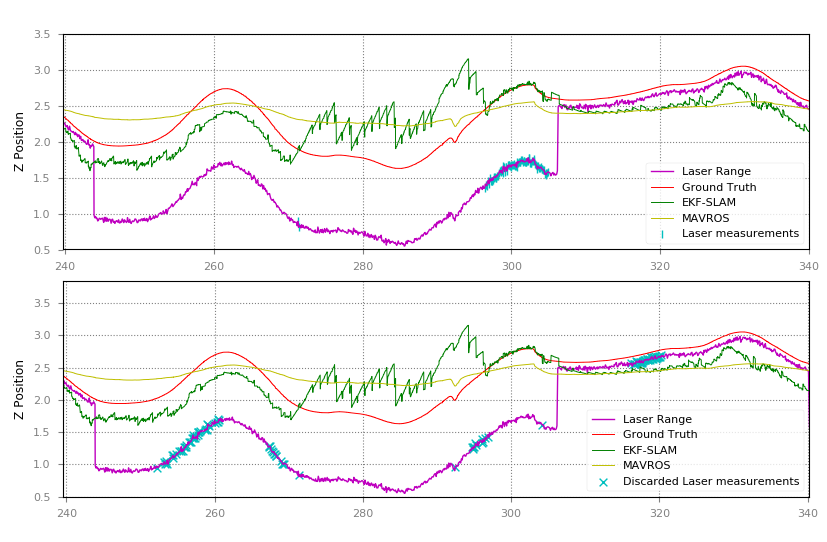
\includegraphics[width=0.9\textwidth]{Images/fig23-laser-chi2-detail.png}
    \caption{Detail of accepted and discarded range sensor observations when $\chi_{\alpha=0.9}^2$}
    \label{fig:chapter3:simulation:c:range-sensor-detail-chi2}
\end{figure}
Similarly, the noisy Octomap measurements and the wrong corrections can be overcome thanks to the \ac{NEES} test. This way, the $\chi^2$ value for one degree of freedom can be reduced in order to accept measurements that are more correlated to those estimated by the filter, hence discarding those noisy Octomap measurements. This procedure can be seen in Figure~\ref{fig:chapter3:simulation:c:range-sensor-chi2}, and the detail in Figure~\ref{fig:chapter3:simulation:c:range-sensor-detail-chi2}. In these plots an acceptance of 0.9 was used, and as shown the discarded measurements are more than in the ones shown in Figure~\ref{fig:chapter3:simulation:c:range-sensor}.\\




















